\bigskip
\section{The Morse Lemma}

We begin by introducing the critical points of a smooth function and the concept of index of a non-degenerate critical point. We will close the section with the first pillar of Morse theory, upon which a large part of the later results will be built: the Morse Lemma.
\medskip
\begin{definition}
    Let $f: $M$ \to \mathbb{R}$ be a smooth function.
    \begin{enumerate}[label=\roman*)]
        \item We will say that $p\in \mathrm{M}$ is a \textit{critical point of $f$} if $d_{p}f:T_{p}M\to \mathbb{R}$ is identically zero. That is, given a local coordinate system $(x_{1}, \dots ,x_{n})$ in a neighborhood $\mathcal{U}$ of $p$ we have
        \begin{equation*}
            \frac{\partial f}{\partial x_1}(p)= \dots = \frac{\partial f}{\partial x_n}(p) = 0.
        \end{equation*}

        \item In turn, we will say that $f(p)\in \mathbb{R}$ is a \textit{critical value of $f$} if $p \in \mathrm{M}$ is a critical point.

    \end{enumerate}
\end{definition}
\bigskip

\begin{definition}
    Let $p\in M$ be a critical point of $f$, we will say that $p$ is \textit{non-degenerate} if the matrix $\left(\frac{\partial^{2}f}{\partial x_i \partial x_j}(p)\right)$ is non-singular, that is, its determinant is non-zero.
\end{definition}
\bigskip

\begin{definition}
    Let $f:M\to \mathbb{R}$ be a smooth function and $p\in M$ a critical point of $f$. We define $\textrm{Hess}_{p}f: T_{p}M\to \mathbb{R}$ as the symmetric bilinear form on the tangent space to $M$ at $p$ constructed as follows: % TRANSLATOR: domain reproduced as in the original; it should be T_pM x T_pM (see IDEAS.md).
    \begin{quote}
        We take $v,w\in T_{p}M$ and let $\tilde{v}$ and $\tilde{w}$ be local extensions of them to vector fields. Then
        \begin{equation*}
            \text{Hess}_{p}f(v,w)=\tilde{v}_{p}(\tilde{w}_{p}(f)),
        \end{equation*}
        where $\tilde{v}_{p}$ is simply $v$ and $\tilde{w}_{p}(f)$ denotes the partial derivative of $f$ in the direction of $\tilde{w}$.
    \end{quote}
\end{definition}
\bigskip
\begin{remark}
    It is quick to check that $\text{Hess}_{p}f$ is indeed symmetric and well defined:

    \begin{enumerate}[label=(\roman*)]
        \item It is symmetric since $\tilde{v}_{p}(\tilde{w}_{p}(f)) - \tilde{w}_{p}(\tilde{v}_{p}(f)) = [\tilde{v},\tilde{w}]_{p}(f) = 0$ where $[\tilde{v},\tilde{w}]$ is the Lie bracket of $\tilde{v}$ and $\tilde{w}$, whose expression in coordinates, let us recall, is
        \begin{equation*}
            [\tilde{v},\tilde{w}]_{p}(f)=\sum_{i=1}^n \big( \tilde{v}_p(\tilde{w}_{i}) - \tilde{w}_p(\tilde{v}_{i}) \big) \left. \frac{\partial}{\partial x_{i}}\right|_p f.
        \end{equation*}
        Hence it vanishes since $p$ is a critical point.

        \item On the other hand, it is well defined since $\tilde{v}_{p}(\tilde{w}_{p}(f))$ does not depend on the chosen extensions of $v$ and $w$, because what matters to us is the vector of the field at the point $p$ and this does not change.
    \end{enumerate}
\end{remark}
\bigskip

Let us now see what $\text{Hess}_pf$ looks like in coordinates. Again, let us take a local coordinate system $(x_{1}, \dots ,x_{n})$, we have
\begin{equation*}
    v=\sum_{i=0}^n a_i \left.\frac{\partial}{\partial x_i}\right|_p ~~\text{and}~~ w=\sum_{i=0}^n b_i \left.\frac{\partial}{\partial x_i}\right|_p . % TRANSLATOR: sums from i=0 reproduced as in the original; they should start at i=1.
\end{equation*}
\medskip

And for the extensions $\tilde{v}$ and $\tilde{w}$ it suffices to take as coefficients the constant functions $a_i$ and $b_j$. Thus

\begin{equation*}
    \text{Hess}_pf= \tilde{v}_{p}(\tilde{w}_{p}(f)) = v\left(\sum_{i=0}^n b_i \left.\frac{\partial}{\partial x_i}\right|_p f\right)=\sum_{i,j} a_ib_i\left.\frac{\partial^{2}}{\partial x_i \partial x_j}\right|_p f . % TRANSLATOR: "a_ib_i" reproduced as in the original; it should be a_ib_j.
\end{equation*}
\medskip

Hence the matrix $\left(\frac{\partial^{2}f}{\partial x_i \partial x_j}(p)\right)$ mentioned before represents the bilinear form $\text{Hess}_pf$ with respect to the basis $\left( \left.\frac{\partial}{\partial x_i}\right|_p,\dots, \left.\frac{\partial}{\partial x_n}\right|_p \right)$ of $T_p\mathrm{M}$.

\vspace{3em}

\begin{definition}
    Let $V$ be a vector space and $H:V\times V\to \mathbb{R}$ a bilinear form on $V$. Then

    \begin{enumerate}[label=\roman*)]
        \item The \textit{index} of $H$ is the maximal dimension of a subspace of $V$ on which $H$ is negative definite.

        \item The \textit{nullity} of $H$ is the dimension of the radical of $H$, that is,
        \begin{equation*}
            \text{dim}(\text{Rad}(H)) ~\text{ with }~ \text{Rad}(H)=\{v\in V:H(v,w)=0, ~\forall w\in V \}.
        \end{equation*}

    \end{enumerate}
\end{definition}


\begin{remark}
    A critical point $p\in M$ of a smooth $f$ is non-degenerate if and only if the nullity of $H=\text{Hess}_pf$ on $T_pM$ is $0$. Indeed:
    \vspace{-2em}
    \begin{quote}
        \mbox{}\\[0.5em]
        $\boxed{\implies}$ Suppose there exists $v\in \text{Rad}(H)$ different from zero, then $H(v,w)=v^tHw=0$ for all $w\in T_pM$, hence $v^tH=0 \text{ if and only if } v^t = 0$ since $H$ is non-singular and $v^tH$ is a linear combination of the rows of $H$, contradiction.

        $\boxed{\impliedby}$ $\text{Rad}(H)=\{0\}$. Suppose that $p$ is degenerate and let $v\in T_pM\setminus\{0\}$, then there exists $w\in T_pM$ such that $v^tHw\neq 0$. Thus, $v^tH\neq 0$ and since $v$ was arbitrary we have that $v^tH\neq 0$ for all $v\in T_pM\setminus\{0\}$, hence $H$ is non-singular and we have reached a contradiction.
    \end{quote}
\end{remark}
\bigskip

\begin{nota}
    From now on we will refer to the bilinear form induced by $f$ as $\text{Hess}_pf$ and to its matrix with respect to the basis of the tangent space as $H_pf$, or simply $H$ if the context allows it. Moreover, we will refer to the index and the nullity of $\text{Hess}_pf$ as the \textit{index and nullity of $f$ at $p$}.
\end{nota}
\bigskip


Now that we have developed the vocabulary to speak about the critical points of a real-valued function, we close this section with the statement and proof of the \textit{Morse Lemma}.

This result is fundamental for the development of Morse theory. Broadly speaking, it establishes that in a neighborhood of a non-degenerate critical point there exists a local coordinate system with respect to which the function $f$ can be expressed as a quadratic form. From a geometric point of view, this implies that $f$ resembles a paraboloid in said neighborhood. This turns out to be incredibly useful and constitutes the basis of the topological arguments we will use from this point on.

\bigskip

Before stating the Morse Lemma we need to prove the following result from differential calculus.

\begin{lemma}
    Let $\mathcal{V}$ be a convex neighborhood of the origin in $\mathbb{R}^n$ and $f\in \mathcal{C}^\infty(\mathcal{V})$ with $f(0)=0$. Then,
    \begin{equation*}
        f(x_1,\dots,x_n)=\sum_{i=1}^n x_ig_i(x_1,\dots,x_n)
    \end{equation*}
    for some functions $g_i\in \mathcal{C}^\infty(\mathcal{V})$ which, moreover, satisfy $g_i(0)=\frac{\partial f}{\partial x_i}(0)$.
\end{lemma}
\begin{proof}
    We have
\begin{align*}
    f(x_i,\dots,x_n)=\int_0^1 \frac{df(tx_1,\dots,tx_n)}{dt}dt = \int_0^1 \big(\sum_{i=1}^n \frac{\partial f}{\partial x_i}&(tx_1,\dots,tx_n)x_i \big)dt =\\
    &=\sum_{i=1}^n x_i \left(\int_0^1 \frac{\partial f}{\partial x_i}(tx_1,\dots,tx_n )dt\right)
\end{align*}

We take $g_i(x_1,\dots,x_n) = \int_0^1 \frac{\partial f}{\partial x_i}(tx_1,\dots,tx_n )dt$ and it holds that $g_i(0)=\int_0^1 \frac{\partial f}{\partial x_i}(0)dt =\frac{\partial f}{\partial x_i}(0)$.

\end{proof}
\bigskip

Let us now proceed with the proof, for which we have relied both on Milnor's (\cite[p.~6]{milnor1963}) and on the one found in \cite[p.~431]{marsdenHoffman1993eca}.

\begin{lemma}[Morse Lemma]\label{lemamorse}
    Let $p$ be a non-degenerate critical point of a smooth function $f:M\to \mathbb{R}$. Then there exists a local coordinate system $(y_1,\dots, y_n)$ in a neighborhood $\mathcal{U}$ of $p$ such that $y_i(p)=0, \forall i\in \{1\dots,n\}$ and
    \begin{equation*}
        f=f(p)-(y_1)^2-\dots-(y_\lambda)^2 + (y_{\lambda +1})^2+\dots + (y_n)^2
    \end{equation*}
    holds on all of $\mathcal{U}$ with $\lambda$ the index of $f$ at $p$.
\end{lemma}
\bigskip

\begin{proof}[Proof of the Morse Lemma]
    %################ PART 1, INDEX ######################
    First of all, let us see that if $f$ can be expressed in that manner on $\mathcal{U}$ then $\lambda$ is necessarily the index of $f$ at $p$. Let $(x_1,\dots, x_n)$ be a local coordinate system on $\mathcal{U}$ and suppose that
    \begin{equation*}
        f=f(p)-(x_i)^2-\dots-(x_\lambda)^2 + (x_{\lambda +1})^2+\dots + (x_n)^2. % TRANSLATOR: "(x_i)^2" reproduced as in the original; it should be (x_1)^2.
    \end{equation*}
    Then we have that

    \[
        \frac{\partial^2 f}{\partial x_i \partial x_j}=
        \begin{cases}
            -2, ~i=j\le \lambda\\
            ~~~2, ~i=j\ge \lambda\\ % TRANSLATOR: overlapping case split reproduced as in the original; the second case should be i=j>lambda.
            ~~~0, i\neq j
        \end{cases}
    \]

    That is, $H_pf$ is a diagonal matrix with $\lambda$ negative values and $n-\lambda$ positive values. Hence it has $\lambda$ negative eigenvalues, which means that there exists a subspace of $T_pM$ of dimension $\lambda$ on which it is negative definite and another of dimension $n-\lambda$ on which it is positive definite.

    The only way in which $\lambda$ could be different from the index of $f$ at $p$ is if there existed a subspace of dimension greater than the one mentioned on which $H_pf$ were negative definite, which is impossible.\\


    %############ PART 2, COORDINATE SYSTEM ##################
    Some preparations are needed before proving that the coordinate system $(y_1,\dots,y_n)$ exists.

    First of all we may assume without loss of generality that, in coordinates, $p$ is the origin of $\mathbb{R}^n$ by composing the chosen chart with the translation taking $p$ to the origin, which is a diffeomorphism. We also assume $f(p)=f(0)=0$; if this were not the case we could take $\bar{f}(q)=f(q)-f(p)$, which satisfies $\bar{f}(p)=0$ and has $p$ as a non-degenerate critical point, and undo the change afterwards.

    By the previous lemma $f(x_1,\dots,x_n)=\sum_{j=1}^n x_jg_j(x_1,\dots,x_n)$ in a convex neighborhood of the origin. Now, since $0$ is a critical point of $f$ we have
    \begin{equation*}
        \frac{\partial f}{\partial x_j}(0)=0 ~\text{ and }~ g_j(0)=\int_0^1 \frac{\partial f}{\partial x_j}(0)~dt=0.
    \end{equation*}
    Hence we can apply the lemma again to each of the $g_j$, obtaining
    \begin{equation*}
        g_j(x_1,\dots,x_n)=\sum_{i=1}^n x_ih_{ij}(x_1,\dots,x_n).
    \end{equation*}
    And, therefore,
    \begin{equation*}
        f(x_1,\dots,x_n)=\sum_{i,j} x_ix_jh_{ij}(x_1,\dots,x_n).
    \end{equation*}
    %here went the quotes part
    Moreover, the matrix $H(0)=(h_{ij}(0))$ is equal to $\frac{1}{2}H_0f=\frac{1}{2}(\frac{\partial^2f}{\partial x_i\partial x_j}(0))$ and is therefore symmetric and non-singular. Indeed, we know that
    \begin{equation*}
        h_{ij}=\int_0^1 \frac{\partial g_i}{\partial x_j}(tx_1,\dots,tx_n)dt ~~\text{ and}~~ g_{i}=\int_0^1 \frac{\partial f}{\partial x_i}(tx_1,\dots,tx_n)dt.
    \end{equation*}
    Hence
    \begin{gather*}
        \frac{\partial g_i}{\partial x_j}(x_1,\dots,x_n)= \int_0^1 \frac{\partial}{\partial x_j}\left(\frac{\partial f}{\partial x_i}(tx_1,\dots,tx_n)\right)dt = \int_0^1 \left(\sum_{k=1}^n\frac{\partial^2 f}{\partial x_i \partial x_k}(tx_1,\dots,tx_n) \frac{\partial(tx_k)}{\partial x_j}\right)dt =\\
        = \int_0^1t\frac{\partial^2 f}{\partial x_i \partial x_j}(tx_1,\dots,tx_n)dt.
    \end{gather*}
    Thus,
    \begin{gather*}
        \frac{\partial g_i}{\partial x_j}(0)=\int_0^1 t\frac{\partial^2 f}{\partial x_i \partial x_j}(0)dt=\frac{\partial^2 f}{\partial x_i \partial x_j}(0)\int_0^1tdt= \frac{1}{2}\frac{\partial^2 f}{\partial x_i \partial x_j}(0)\implies\\
        \implies h_{ij}(0)=\frac{1}{2}\frac{\partial^2 f}{\partial x_i \partial x_j}(0)\int_0^1 dt =\frac{1}{2}\frac{\partial^2 f}{\partial x_i \partial x_j}(0)
    \end{gather*}
    %############### INDUCTION ###########################
    Finally, we have $f$ expressed similarly to a quadratic form. What we want to do next is diagonalize it, and to that end we will proceed by induction.

    The base case of the induction ($r=1$) is already proven.

    Suppose now that there exists a coordinate system $(u_i,\dots,u_n)$ in a neighborhood $\mathcal{U}_1$ of $0$, perhaps smaller than $\mathcal{U}$, such that % TRANSLATOR: "(u_i,...,u_n)" reproduced as in the original; it should be (u_1,...,u_n).
    \begin{equation}
        f = \pm (u_1)^2 \pm\dots\pm (u_{r-1})^2 + \sum_{i,j\ge r} u_i u_j H_{ij}(u_1,\dots,u_n)
    \label{eq1}
    \end{equation}
    on all of $\mathcal{U}_1$ with $r > 1$ and $H_{ij}=H_{ji}$ for any $i$ and $j$.

    We can now perform a linear change of coordinates in $(u_r,\dots, u_n)$ to diagonalize $\sum_{i,j\ge r} u_i u_j H_{ij}(0)$.

    We know that, the matrix $(H_{ij})$ being non-singular, the terms of the diagonal are all non-zero. Hence we may assume $H_{rr}\neq 0$. Let $g(u_1,\dots,u_n)=|H_{rr}(u_1,\dots,u_n)|^{1/2}$; it is clear that there exists a neighborhood $\mathcal{U}_2\subset \mathcal{U}_1$ of $0$ on which it is smooth and does not vanish. We define the new coordinate system
    \begin{equation}
        \begin{cases}
            V_i(u_1,\dots,u_n) = u_i,~~i\neq r\\
            V_r(u_1,\dots,u_n)=g(u_1,\dots,u_n)\left[u_r+\sum_{i>r}u_i\frac{H_{ir}(u_1,\dots,u_n)}{H_{rr}(u_1,\dots,u_n)}\right],
        \end{cases}
    \label{eq2}
    \end{equation}

    let us see that it is indeed one. We have that the Jacobian matrix of the coordinate transformation at $0$ is
    \begin{equation*}
        \frac{\partial (V_1,\dots, V_n)}{\partial (u_1,\dots, u_n)} =
        \begin{pmatrix}
            1 & 0 & ~ & \dots & ~ & ~ & 0 \\
            0 & ~ & ~ & ~ & ~ & ~ & 0 \\
            \vdots & ~ & 1 & ~ & ~ & ~ & \vdots \\
            \frac{\partial V_r}{\partial u_1} & \dots & ~ & g(0) & ~ & \dots & \frac{\partial V_r}{\partial u_n} \\
            0 & ~ & ~ & ~ & 1 & ~ & 0 \\
            \vdots & ~ & ~ & ~ & ~ & ~ & \vdots \\
            0 & ~ & ~ & \dots & ~ & 0 & 1
        \end{pmatrix},
    \end{equation*}
    and it is non-singular: it suffices to subtract from the $r$-th row the other rows multiplied by the appropriate term $\frac{\partial V_i}{\partial u_j}$ so that it becomes diagonal, and the terms of the diagonal are all non-zero.

    It then follows from the \textit{inverse function theorem} that the transformation is a diffeomorphism on a smaller neighborhood $\mathcal{U}_3\subset \mathcal{U}_2$ of $0$ and therefore $(v_1,\dots, v_n)$ is a local coordinate system around $p$.

    \bigskip

    We now consider
    \begin{equation}
        u_ru_rH_{rr}(u_1,\dots, u_n) + 2\sum_{j=r+1}^n u_ju_rH_{jr}(u_1,\dots, u_n).
    \label{eq3}
    \end{equation}

    Using the symmetry of $H_{ij}$ we observe that this expression is nothing but the terms of \eqref{eq1} having $j=r$ or $i=r$. Comparing \eqref{eq1} and \eqref{eq2} we arrive at the fact that \eqref{eq3} is
    \begin{equation}
        \pm V_rV_r - \frac{1}{H_{rr}}\left[ \sum_{i>r} u_iH_{ir}(u_1,\dots, u_n) \right]^2
    \label{eq4}
    \end{equation}

    Indeed,

    \begin{align*}
        V_rV_r =& ~ g^2 \left[u_r+\sum_{i>r}u_i\frac{H_{ir}}{H_{rr}}\right]^2 =\\
        =& ~ g^2 \left( u_r^2 + \left[ \sum_{i>r}u_i\frac{H_{ir}}{H_{rr}}\right]^2 + 2u_r\sum_{i>r}u_i\frac{H_{ir}}{H_{rr}} \right) = \\
        =& ~ |H_{rr}| u_r^2 + \frac{|H_{rr}|}{H_{rr}^2} \left[\sum_{i>r}u_iH_{ir}\right]^2 + 2u_r\frac{|H_{rr}|}{H_{rr}}\sum_{i>r}u_iH_{ir} = \\
        =& ~ \pm H_{rr}u_r^2 \pm \frac{1}{H_{rr}}\left[\sum_{i>r}u_iH_{ir}\right]^2 \pm 2u_r\sum_{i>r}u_iH_{ir},
    \end{align*}

    \vspace{2em}

    where the $\pm$ will be $+$ if $H_{rr}$ is positive and $-$ if it is negative, and likewise in \eqref{eq4}.
    \bigskip

    Thus, it is clear that \eqref{eq3} and \eqref{eq4} are equivalent. And from here it is easy to see how \eqref{eq1} turns into
    \begin{equation*}
        f = \pm (V_1)^2 \pm\dots\pm (V_{r-1})^2 + (V_r)^2  \pm \sum_{i,j > r} V_iV_j\tilde{H}_{ij}(V_1,\dots,V_n)
    \end{equation*}
    for some new symmetric terms $\tilde{H}_{ij}$ in terms of the new coordinate system.

    This concludes the induction, since we have one more quadratic summand, and the existence of the sought local coordinate system is proven.

\end{proof}

\bigskip

\begin{remark}
    A part of the process remains implicit throughout the proof. When defining the new coordinate system in the induction step, what we are doing is defining a function we may call $l:\mathbb{R}^n \to \mathbb{R}^n$ that, given the coordinates $(u_1(p),\dots, u_n(p))$ of a point $p\in M$, takes them to new ones $(v_1(p),\dots, v_n(p))$ and is a diffeomorphism between open sets of $\mathbb{R}^n$. Thus, if the chart inducing the coordinate system $(u_1,\dots, u_n)$ was $\varphi : M \to \mathbb{R}^n$, the one inducing $(v_1,\dots, v_n)$ will be $l\circ \varphi$.
\end{remark}
\bigskip

The following corollary will be key when proving one of the main theorems of Morse theory (see \ref{cwvariedad}) and shows one of the fundamental advantages of working with non-degenerate critical points.
\bigskip
\begin{corollary}
        Let $M$ be a smooth manifold. Every non-degenerate critical point of a smooth function from $M$ to $\mathbb{R}$ is isolated from the other critical points.
\end{corollary}
\begin{proof}
    Let $p\in M$ be a non-degenerate critical point of a function $f$. There exists a local coordinate system $(y_1,\dots, y_n)$ in a neighborhood $\mathcal{U}$ of $p$ such that $y_i(p)=0$ for all $i\in\{1,\dots,n\}$ and
    \begin{equation*}
        f=f(p)-(y_i)^2-\dots-(y_\lambda)^2 + (y_{\lambda +1})^2+\dots + (y_n)^2 % TRANSLATOR: "(y_i)^2" reproduced as in the original; it should be (y_1)^2.
    \end{equation*}
    by the Morse Lemma (\ref{lemamorse}).

    Suppose there exists another critical point $q\in\mathcal{U}$, then
    \begin{equation*}
        \frac{\partial f}{\partial x_i}(q)=\pm 2q_i= 0\iff q_i= y_i(q)=0\iff q_i=p_i
    \end{equation*}
    Hence $p$ is the only critical point of $f$ in $\mathcal{U}$.

\end{proof}
\bigskip

Next we present some degenerate and non-degenerate critical points together with the graphs of their corresponding functions, Figures \ref{fig:ptos_criticos1}, \ref{fig:ptos_criticos2} and \ref{fig:ptos_criticos3}. Observe that while non-degenerate points must be isolated, a function can have degenerate critical points that are either isolated or non-isolated.
\begin{example}
    \hfil
    \begin{enumerate}
        \item The function $f(x,y)=(x^2-1)^2 + (y^2-1)^2$ has nine non-degenerate critical points. It is easy to check that $\text{Hess}_pf$ is a diagonal matrix whose entries do not vanish at any of the critical points.
        \item The function $g(x,y)=x^3-3xy^2$, whose graph corresponds to the ``monkey saddle'', possesses a single degenerate critical point at the point $(0,0)$. It suffices to see that $\text{Hess}_{(0,0)}f$ has zeros in all four entries. % TRANSLATOR: "f" reproduced as in the original; it should be g.
        \item We observe that $h(x,y)= x^2y^2$ has infinitely many degenerate critical points, those of the form $(0,y)$ and $(x,0)$.
    \end{enumerate}
\end{example}

\begin{figure}[H]
\begin{minipage}{0.35\textwidth}
    \centering
    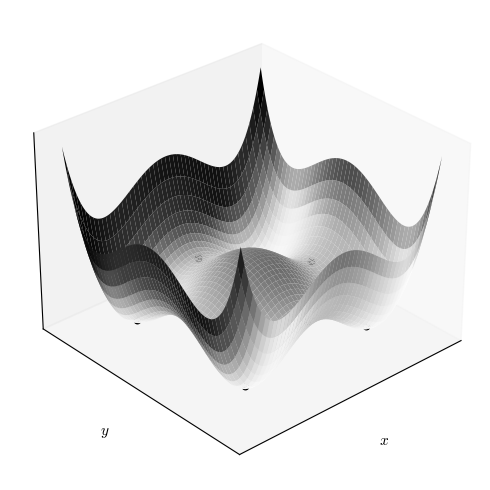
\includegraphics[width=\textwidth]{imagenes/grafica1.png}
    \caption{$f(x,y)=(x^2-1)^2 + (y^2-1)^2$}
    \label{fig:ptos_criticos1}
\end{minipage}
\hfill
\begin{minipage}{0.35\textwidth}
    \centering
    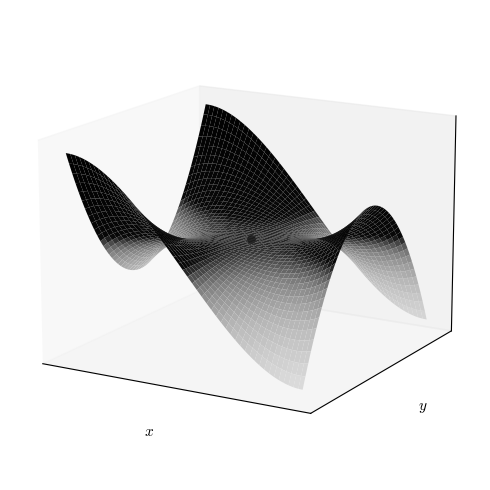
\includegraphics[width=\textwidth]{imagenes/grafica2.png}
    \caption{$g(x,y)=x^3-3xy^2$}
    \label{fig:ptos_criticos2}
\end{minipage}

% --- Second row ---
\centering
\begin{minipage}{0.35\textwidth}
    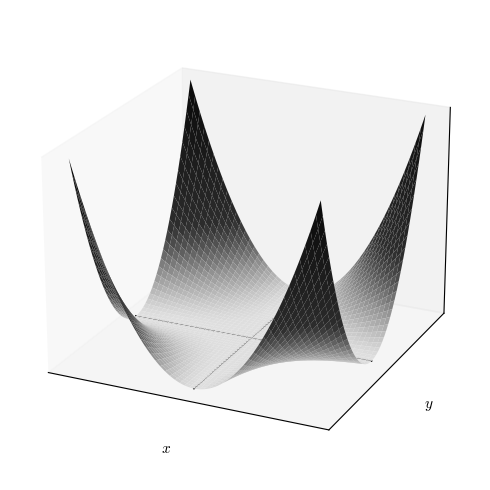
\includegraphics[width=\textwidth]{imagenes/grafica3.png}
    \caption{$h(x,y)= x^2y^2$}
    \label{fig:ptos_criticos3}
\end{minipage}

\end{figure}

We conclude the chapter by defining the objects that give it its name and of which we will make use from now on to describe the CW-complex structure of any smooth manifold.
\bigskip

\begin{definition}
 We will say that a smooth function $f: M\to \mathbb{R}$ is a \textit{Morse function} if all its critical points are non-degenerate.
\end{definition}

\iffalse
{\color{blue} Prove that for every finite-dimensional manifold there exists a Morse function?}
\fi
